\section{Interactive Features}
\label{sec:interactive_features}

\subsection{Dynamically updating legend}

The legend displayed at the bottom left shows the names of layers being visualized next to representative icons. For layers with gradient attributes, the legend icon shows the gradient scale, and the name indicates the attribute being visualized along with associated units. 

The legend details update dynamically as layers are selected, de-selected and customized.

\subsection{Dropdown for area layer selection}

Area layers can be selected one at a time for visualization using the dropdown menu at the top. The constraint to only view one area feature at a time is imposed to avoid potential confusion from overlapping features blocking each other out. 

\begin{figure}[ht]
        \centering
        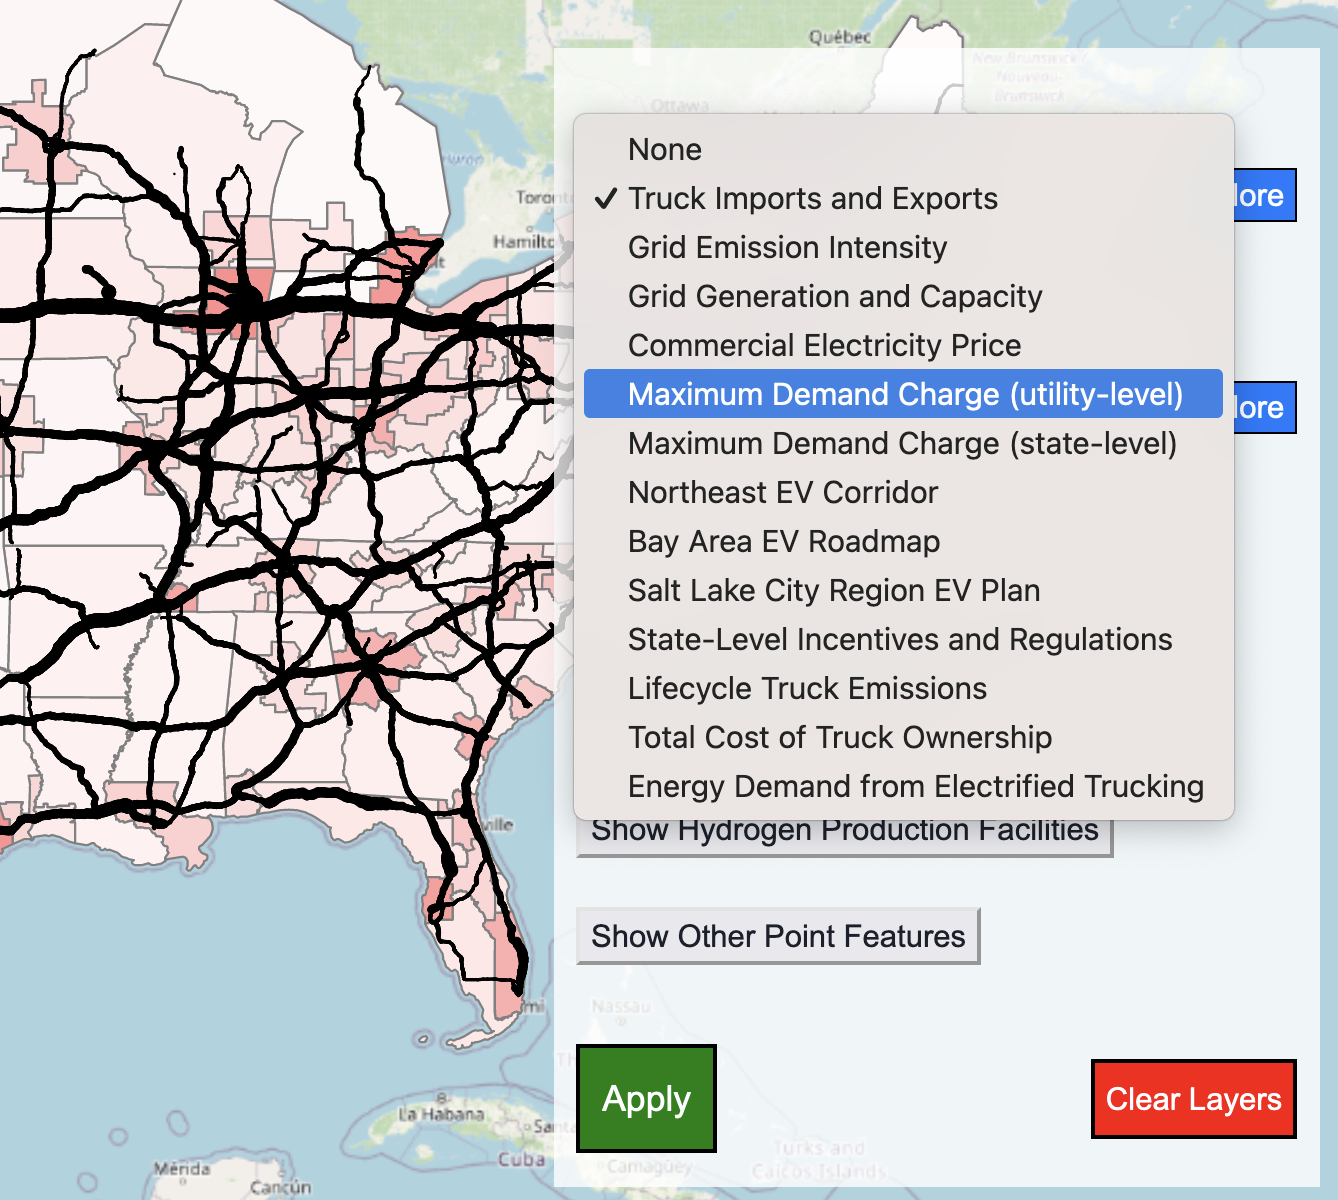
\includegraphics[width=0.5\textwidth]{figures/dropdown_area.png}
        \caption{Dropdown menu used for area layer selection}
        \label{fig:dropdown_area}
\end{figure}

\subsection{Multiple-choice highway and point layer selection}

Any number of highway and point layers can be visualized simultaneously, since overlap confusion is less of a concern with these layer types. 

Layers to visualize are selected with checkboxes. To avoid cluttering the interface,  checkboxes and associated layer names are hidden by default. Different classes of layers (eg. highway flows, planned infrastructure corridors, etc.) can be expanded for viewing and selection by clicking on the associated 'show' button (eg. 'Show Highway Flows'). 

\begin{figure}[ht]
        \centering
        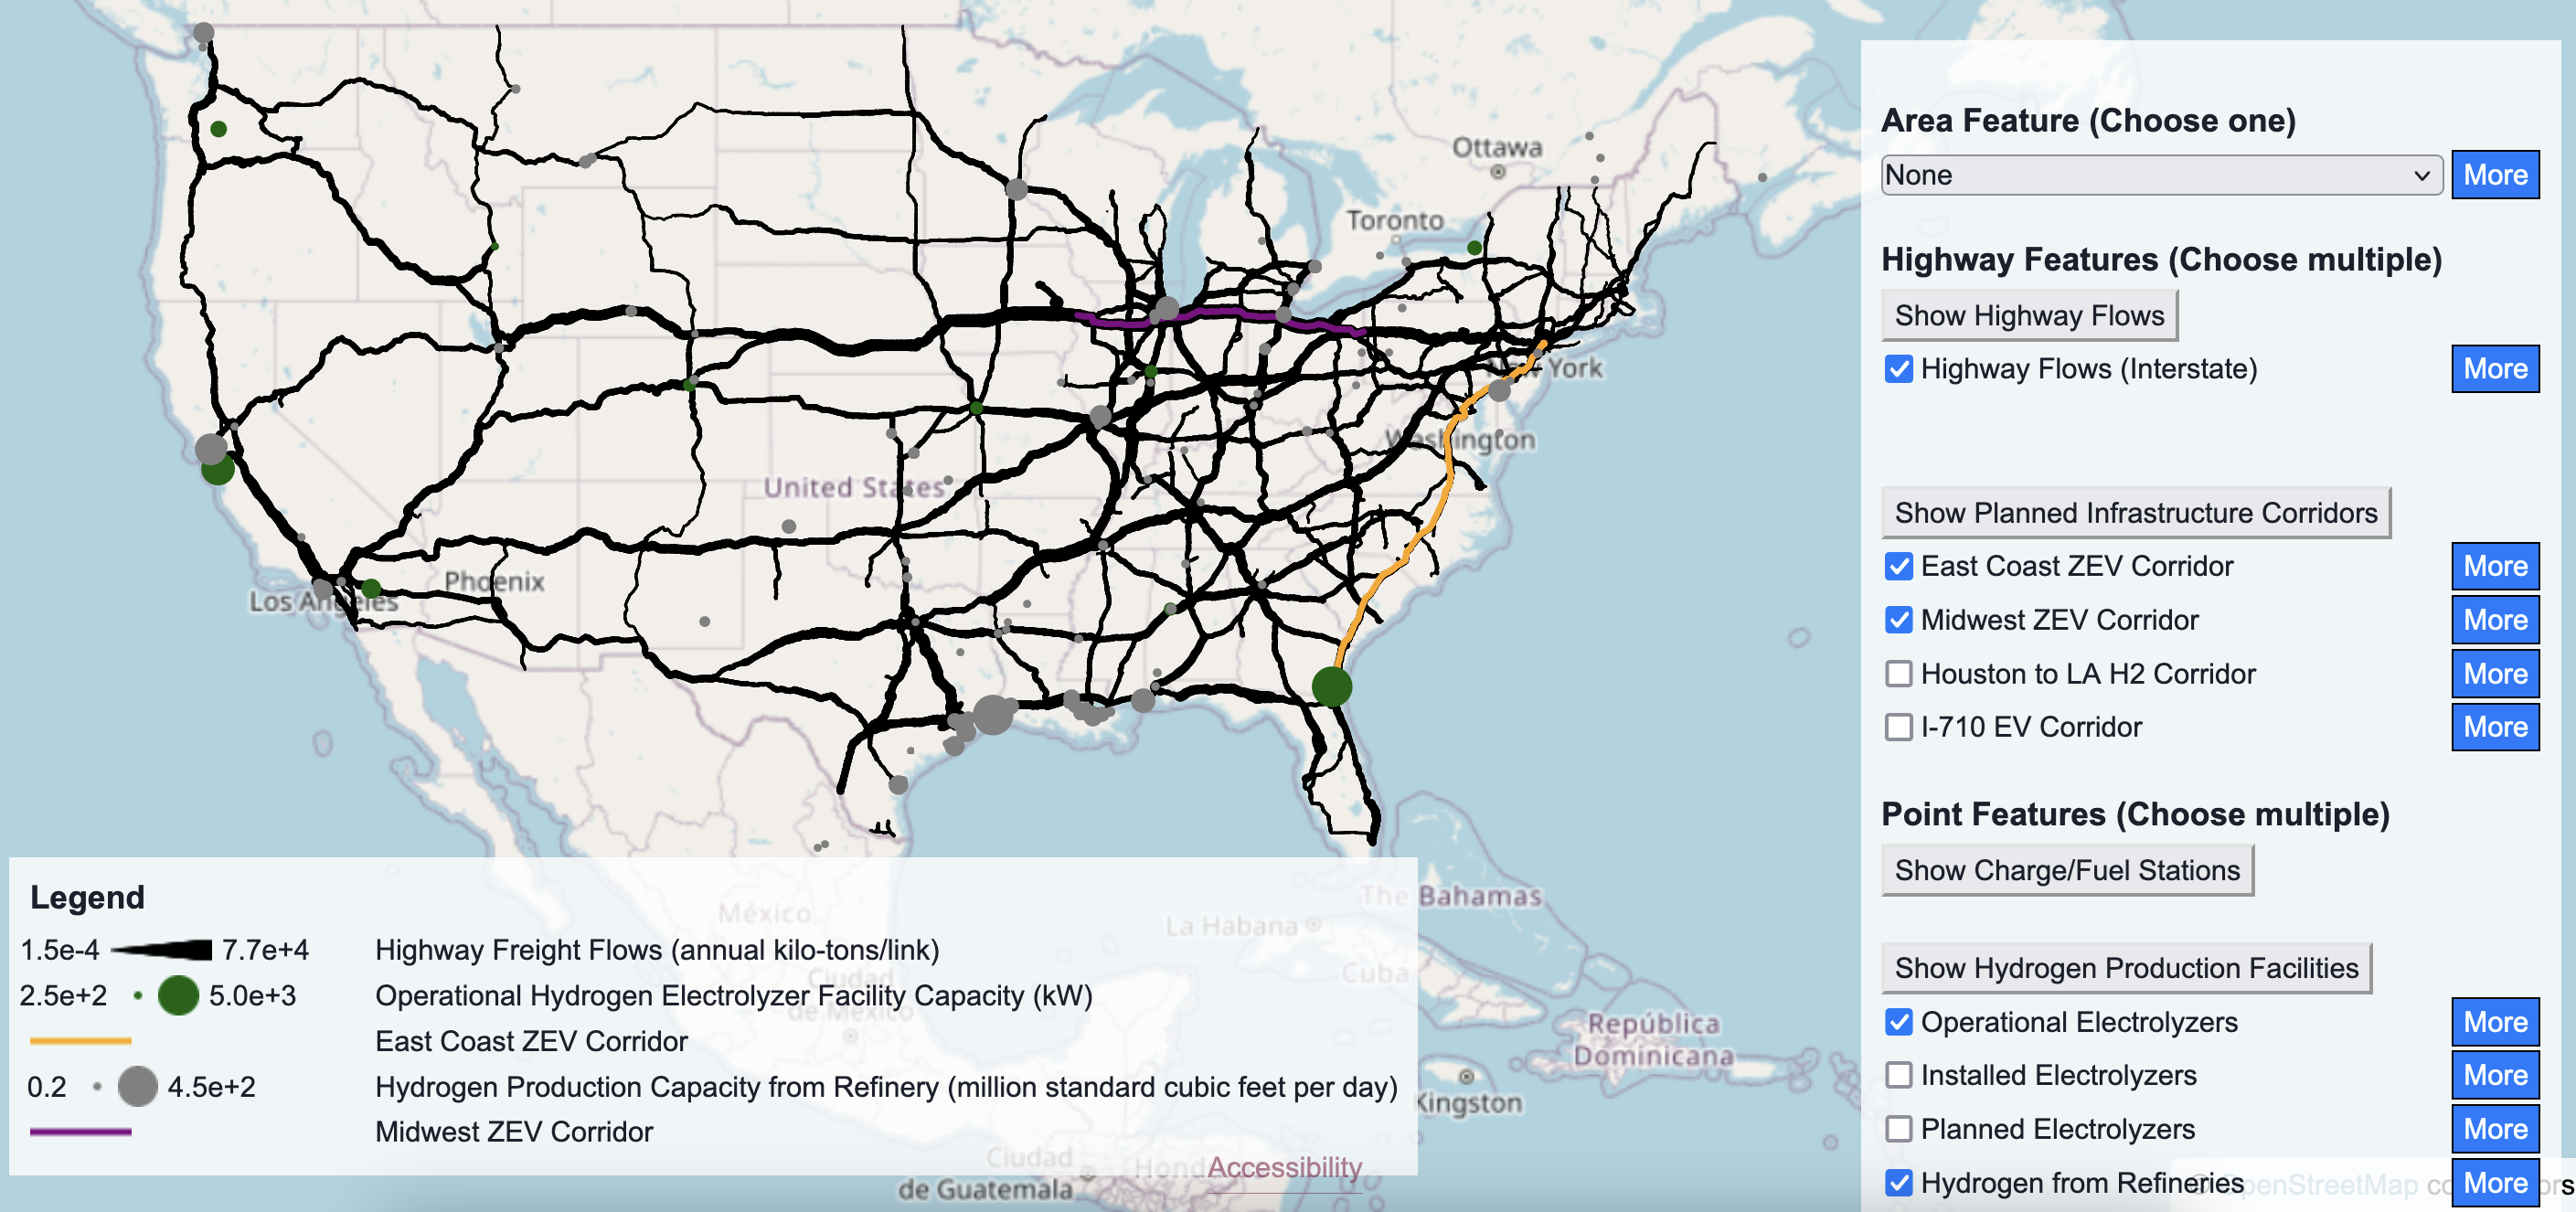
\includegraphics[width=0.9\textwidth]{figures/checkboxes.png}
        \caption{Checkboxes are used to visualize several point and highway layers simultaneously.}
        \label{fig:checkboxes}
\end{figure}

\subsection{Pop-up window for data sources and layer gradient customization}

Each layer in the interface has a blue 'More' button to the right of it. Clicking the 'More' button next to a given layer opens a pop-up window with the following information:

\begin{itemize}
    \item Information on the data source(s), including links to the original raw data whenever possible. In cases where analysis or synthesis is performed to produce the visualized quantity, the methodology involved is briefly described, and the associated analysis code is linked to where appropriate.
    \item A link to download the geojson file used to visualize the geospatial data. 
    \item For some layers, the user can customize details of the displayed gradient attribute. For such layers, the pop-up window includes one or more dropdown menus for this customization.
\end{itemize}

\begin{figure}[ht]
        \centering
        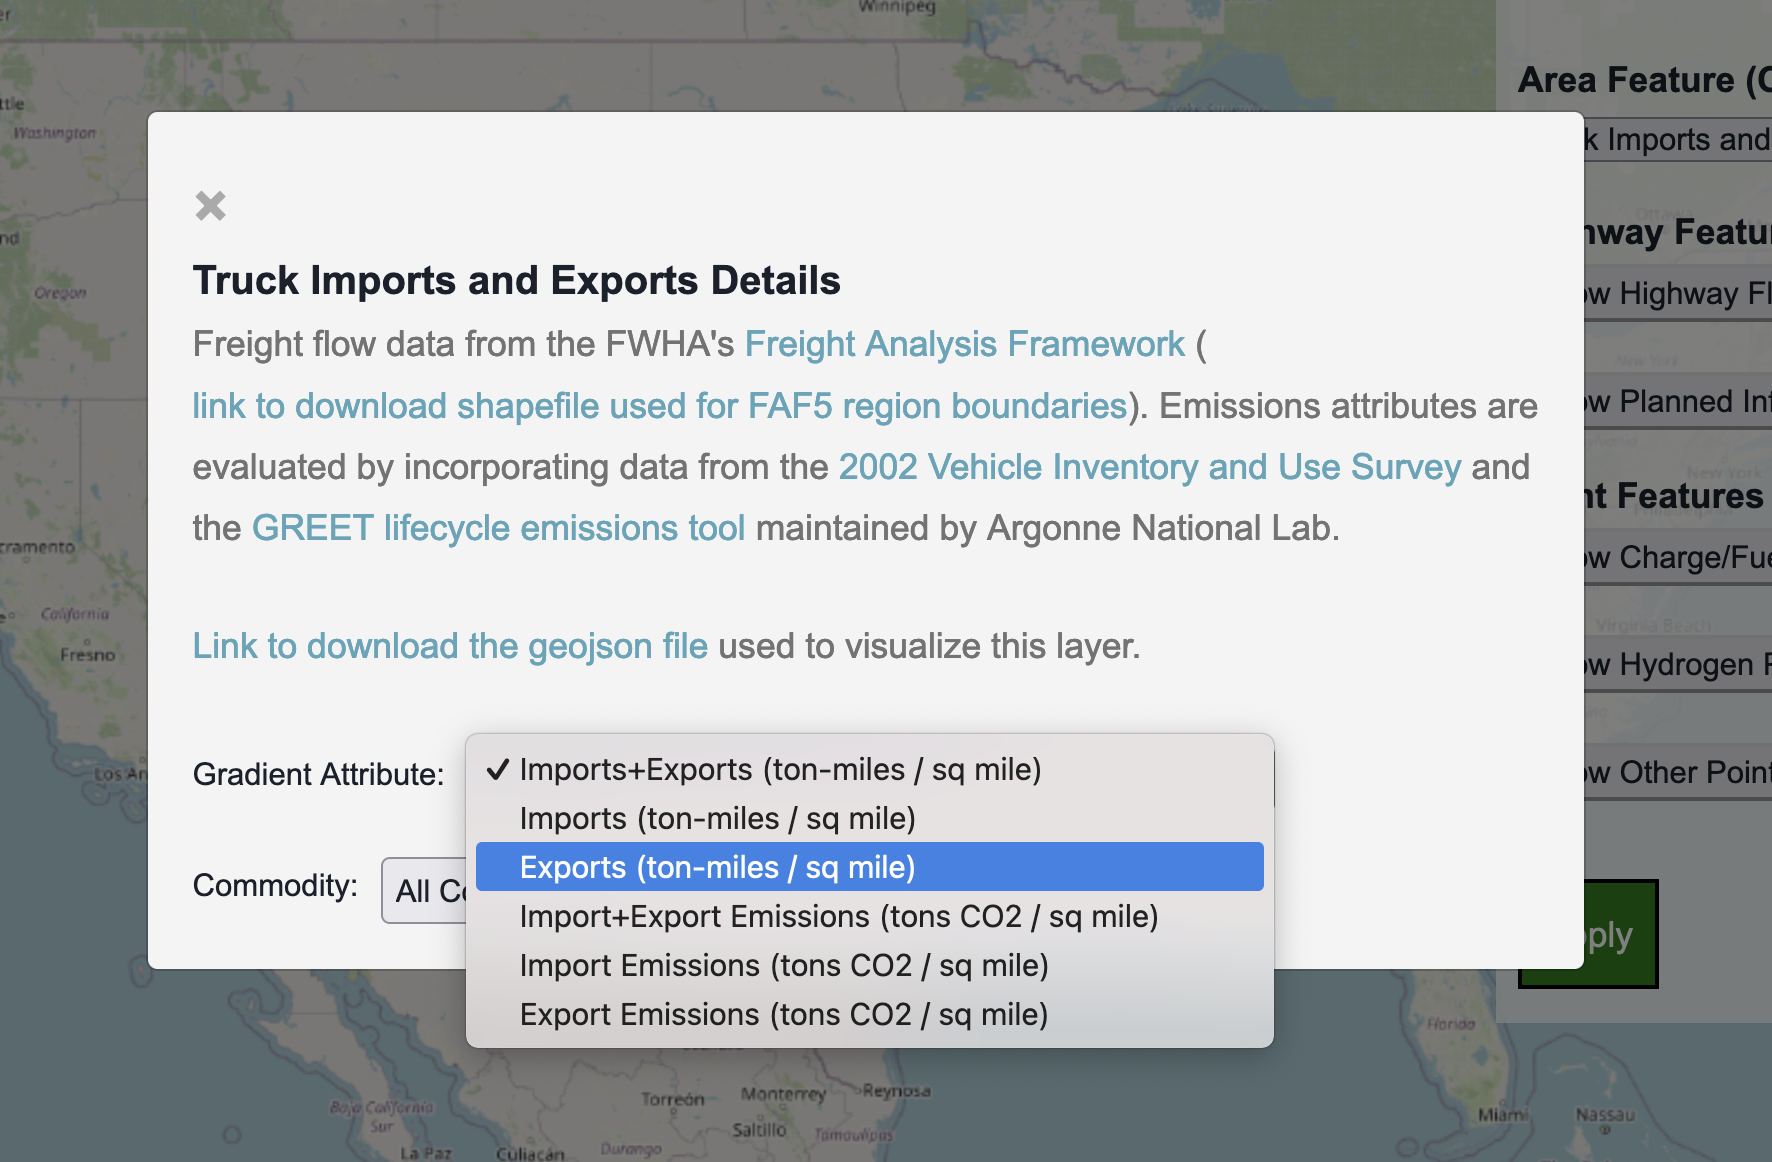
\includegraphics[width=0.7\textwidth]{figures/popup_dropdown.png}
        \caption{Dropdown menus to customize details of the areal freight flow density.}
        \label{fig:popup_dropdown}
\end{figure}